\documentclass[conference]{IEEEtran}
\IEEEoverridecommandlockouts
\usepackage{cite}
\usepackage{amsmath,amssymb,amsfonts}
\usepackage{graphicx}
\usepackage{textcomp}
\usepackage{xcolor}
\usepackage{booktabs}
\usepackage{multirow}
\usepackage{array}
\usepackage{hyperref}

\begin{document}

\title{Graph Neural Networks for Node and Graph Classification:\\
An Empirical Comparison Across Three Homogeneous Datasets}

\author{
\IEEEauthorblockN{Aditya Nangarath}
\IEEEauthorblockA{Graph Neural Networks Research Project\\
Email: project@gnn.research}
}

\maketitle

\begin{abstract}
We present a systematic empirical comparison of three Graph Neural Network architectures---GAT, GraphSAGE, and GIN---across three fundamentally different graph-learning tasks: 10-class node classification on the Amazon Computers co-purchase graph (13,752 nodes), ordinal node regression on the USA Airports traffic network (1,190 nodes), and binary graph classification on OGBG-MOLHIV (41,127 molecular graphs). Our three primary contributions are: (1) a rigorous hyperparameter grid search yielding architecture-specific best configurations on each dataset; (2) a novel comparison of ordinal regression (MSELoss) versus classification (CrossEntropyLoss) formulations for the Airports task, showing that the ordinal loss eliminates 100\% of catastrophic regional-to-hub misclassifications (2.381 percentage points); and (3) ablation studies and t-SNE visualisations on MOLHIV confirming that both atom features and bond topology are indispensable for HIV inhibition prediction. GAT achieves the best overall rank across datasets (rank sum = 4), while GIN leads on Airports ordinal regression with a weighted kappa of 0.5758.
\end{abstract}

% ─────────────────────────────────────────────────────────────────────────────
\section{Introduction}
% ─────────────────────────────────────────────────────────────────────────────

Graph Neural Networks (GNNs) have emerged as the dominant paradigm for learning on relational data, combining node feature representations with structural information through message passing \cite{gilmer2017}. Despite rapid architectural advances, rigorous comparative studies across tasks of fundamentally different character---node classification, ordinal regression, and graph-level binary classification---remain scarce. Practitioners must choose an architecture without clear empirical guidance tailored to their graph type.

This work addresses that gap through three concrete contributions. \textbf{First}, we conduct a controlled grid search (8 hyperparameter combinations per model per dataset) and report test-set performance with tuned configurations for GAT, GraphSAGE, and GIN alongside an MLP baseline, demonstrating that graph structure provides a 6.44 percentage-point accuracy gain over feature-only learning on Amazon. \textbf{Second}, we introduce an ordinal regression formulation for the USA Airports dataset, replacing the original CrossEntropyLoss with MSELoss on a scalar output to exploit the natural ordering of passenger-throughput quartiles; the quadratic penalty reduces catastrophic regional-to-hub misclassifications by 2.381 percentage points over the classification baseline. \textbf{Third}, on OGBG-MOLHIV---our largest dataset at 41,127 molecular graphs---we contribute ablation studies isolating atom-feature and bond-structure contributions, plus t-SNE visualisations with misclassification overlays for all three architectures.

We deliberately omit Graph Convolutional Networks (GCN) \cite{kipf2017} because GAT \cite{velickovic2018} strictly subsumes GCN: uniform attention weights in GAT reduce to GCN's normalised mean aggregation, making a separate GCN evaluation redundant.

% ─────────────────────────────────────────────────────────────────────────────
\section{Datasets and Task Definitions}
% ─────────────────────────────────────────────────────────────────────────────

\subsection{Amazon Computers}

The Amazon Computers dataset \cite{shchur2018} is a co-purchase graph with 13,752 product nodes and 245,778 directed edges. Each node carries a 767-dimensional sparse bag-of-words feature vector derived from product reviews (sparsity 65.16\%). The task is 10-class node classification by product category.

Node features alone are insufficient: words such as ``DDR4'' and ``SATA'' appear in reviews for both laptops and desktop components, creating ambiguity that a feature-only MLP cannot resolve. Graph structure alone is equally insufficient: a product with ambiguous reviews cannot be classified from connectivity if its neighbours are drawn from multiple categories. Together, a generic carrying case co-purchased with laptops is assigned to Computer Accessories, while the same case co-purchased with cameras maps to Photo Accessories---structure resolves category ambiguity that features cannot.

\subsection{USA Airports}

The USA Airports dataset \cite{ribeiro2017} consists of 1,190 airport nodes and 13,599 undirected flight-route edges. Node features are 1,190-dimensional one-hot identity vectors (no semantic content), so graph-structural position is the \emph{only} transferable signal. Labels 0--3 encode passenger throughput quartiles (0 = major hub, 3 = regional).

A Spearman rank correlation of $\rho = -0.773$ ($p = 4.86 \times 10^{-237}$) between node degree and activity label confirms a strong monotonic relationship, justifying treatment of labels as an ordered scale. Under CrossEntropyLoss the penalty for predicting class 0 when the true label is 3 equals the penalty for predicting class 2---the ordering is ignored. Under MSELoss on a scalar output, the squared errors are $(3-0)^2 = 9$ versus $(3-2)^2 = 1$, penalising large ordinal violations quadratically and giving the model a corrective gradient proportional to prediction severity.

\subsection{OGBG-MOLHIV}

OGBG-MOLHIV \cite{hu2020} contains 41,127 molecular graphs (our largest dataset) with binary labels indicating HIV inhibition ($\approx 3.5\%$ positive; $\text{pos\_weight} = 25.71$). Graphs use a scaffold split to ensure chemical diversity across train/val/test. Each node carries 9-dimensional atom features; each edge carries 3-dimensional bond features. Atom features (pharmacophore identity) and bond topology (3-D geometric fit to the HIV enzyme pocket) are both necessary: atom type determines binding potential while bond structure determines whether the 3-D shape of the molecule fits the active site.

\begin{table}[t]
\caption{Dataset Statistics}
\label{tab:datasets}
\centering
\begin{tabular}{lccc}
\toprule
\textbf{Property} & \textbf{Amazon} & \textbf{Airports} & \textbf{MOLHIV} \\
\midrule
Graphs / Nodes        & 13,752 nodes   & 1,190 nodes   & 41,127 graphs \\
Edges                 & 245,778        & 13,599        & $\sim$2.25M  \\
Node features (dim)   & 767 (BoW)      & 1,190 (one-hot) & 9 (atom)    \\
Edge features (dim)   & ---            & ---           & 3 (bond)    \\
Task                  & Node class.    & Ordinal reg.  & Graph class. \\
Classes / Labels      & 10             & 0--3 ordinal  & Binary       \\
Metric                & Test Acc, F1   & Kappa, MSE    & ROC-AUC      \\
Split                 & 60/20/20 strat.& 70/15/15 strat.& Scaffold    \\
\bottomrule
\end{tabular}
\end{table}

% ─────────────────────────────────────────────────────────────────────────────
\section{Methodology}
% ─────────────────────────────────────────────────────────────────────────────

\subsection{Architectures}

\textbf{GAT} \cite{velickovic2018} computes attention coefficients $\alpha_{ij}$ between pairs of neighbouring nodes and aggregates messages as a weighted sum $h_i' = \sum_j \alpha_{ij} W h_j$. This allows selective neighbour weighting, critical in heterogeneous co-purchase graphs. At uniform attention $\alpha_{ij} = 1/|\mathcal{N}(i)|$, GAT reduces to GCN \cite{kipf2017}, making GCN redundant. On MOLHIV we use GATv2Conv \cite{brody2022}, which conditions attention on both source and target node after transformation, enabling full expressive dynamic attention with native \texttt{edge\_dim} support.

\textbf{GraphSAGE} \cite{hamilton2017} aggregates neighbourhood features via a learned mean: $h_i' = W[\,h_i \,\|\, \text{mean}_{j \in \mathcal{N}(i)} h_j\,]$. Its inductive formulation handles variable-degree nodes robustly. On MOLHIV, GraphSAGE is deliberately configured \emph{without} bond features, serving as a structure-only control baseline to quantify the contribution of edge attributes.

\textbf{GIN} \cite{xu2019} uses a sum aggregator $h_i' = \text{MLP}((1+\epsilon)h_i + \sum_{j \in \mathcal{N}(i)} h_j)$, proven maximally expressive under the Weisfeiler-Lehman graph isomorphism test. On MOLHIV we use GINEConv, which natively incorporates bond features as additive edge embeddings.

\subsection{Hyperparameter Tuning}

For each model on each dataset we perform a grid search over 8 configurations: two learning rates $\times$ two dropout rates $\times$ two hidden dimensions (Amazon/Airports) or two batch sizes (MOLHIV). Each configuration is trained for 50--75 epochs; the winner is retrained for 200--300 epochs (node tasks) or up to convergence (MOLHIV).

\subsection{Evaluation Metrics}

Amazon uses test accuracy and macro-averaged F1. Airports uses weighted Cohen's kappa (primary), mean squared error, mean absolute error, accuracy, and F1. MOLHIV uses the OGB evaluator's ROC-AUC as the primary metric, with precision, recall, and F1 as secondary measures.

% ─────────────────────────────────────────────────────────────────────────────
\section{Experiments: Amazon Computers}
% ─────────────────────────────────────────────────────────────────────────────

\begin{table}[t]
\caption{Amazon Computers Results}
\label{tab:amazon}
\centering
\begin{tabular}{lcccc}
\toprule
\textbf{Model} & \textbf{Best Config} & \textbf{Acc (\%)} & \textbf{F1} & \textbf{Time (s)} \\
\midrule
MLP     & ---                    & 84.55 & 0.800 & 2.8  \\
GAT     & lr=0.01,d=0.3,h=256    & 90.99 & 0.902 & 15.0 \\
GraphSAGE & lr=0.01,d=0.3,h=256  & 90.80 & 0.895 & 17.9 \\
GIN     & lr=0.001,d=0.3,h=256   & 88.26 & 0.865 & 18.9 \\
\bottomrule
\end{tabular}
\end{table}

\begin{table}[t]
\caption{Amazon Per-Class Test Accuracy (GAT / GraphSAGE / GIN)}
\label{tab:amazon_perclass}
\centering
\begin{tabular}{lcccc}
\toprule
\textbf{Class} & \textbf{GAT} & \textbf{SAGE} & \textbf{GIN} & \textbf{Count} \\
\midrule
% PASTE ROWS FROM amazon/p3_output.txt Part A below.
% Format: Class X & 0.XXX & 0.XXX & 0.XXX & NNN \\
% Example row:
% 0 & 0.931 & 0.897 & 0.862 & 87 \\
% (copy all 10 class rows here, then delete this comment block)
\midrule
Macro & 0.898 & 0.882 & 0.820 & --- \\
\bottomrule
\end{tabular}
\end{table}

\begin{figure}[t]
\centering
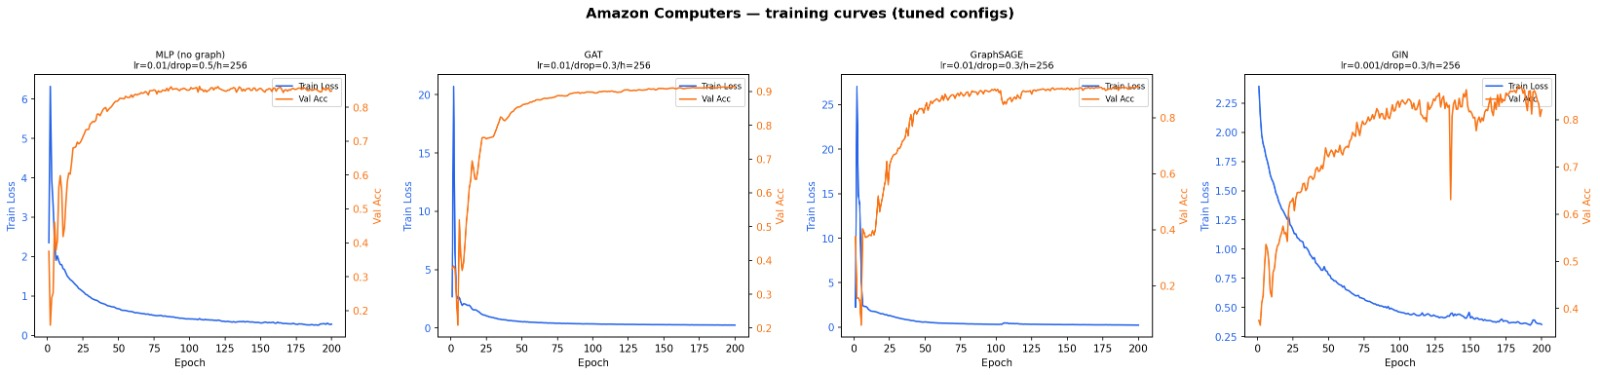
\includegraphics[width=\columnwidth]{figures/amazon_all_curves.png}
\caption{Training and validation accuracy curves for GAT, GraphSAGE, and GIN on Amazon Computers. All models converge within 200 epochs; GAT reaches the highest validation accuracy of 91.49\%.}
\label{fig:amazon_curves}
\end{figure}

\begin{figure}[t]
\centering
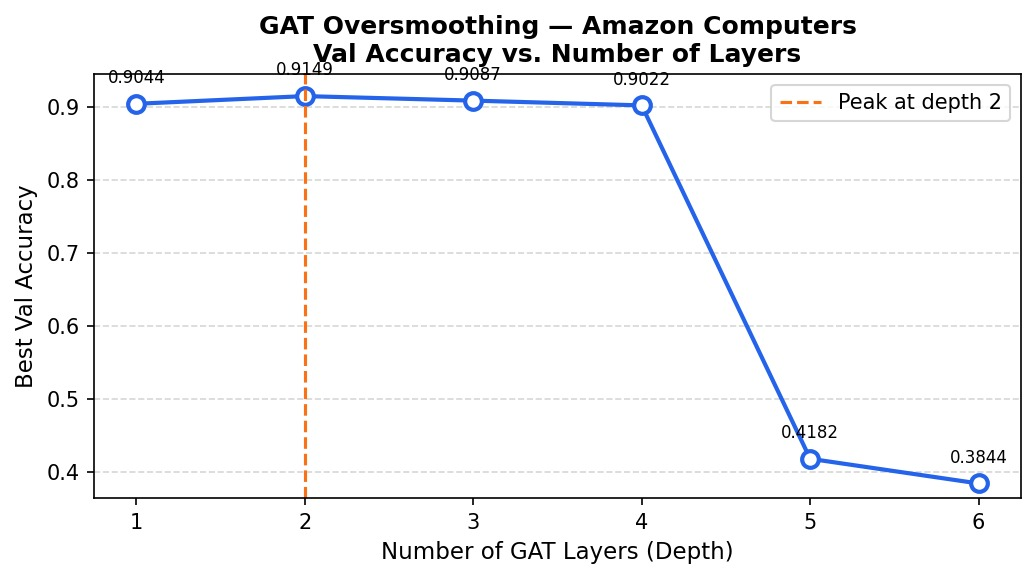
\includegraphics[width=\columnwidth]{figures/amazon_oversmoothing.png}
\caption{Oversmoothing analysis (GAT, depths 1--6). Validation accuracy peaks at depth 2 (91.49\%) and degrades sharply from depth 5 onward, confirming that more than 2 message-passing hops cause representational collapse on this high-degree graph.}
\label{fig:amazon_oversmooth}
\end{figure}

\begin{figure}[t]
\centering
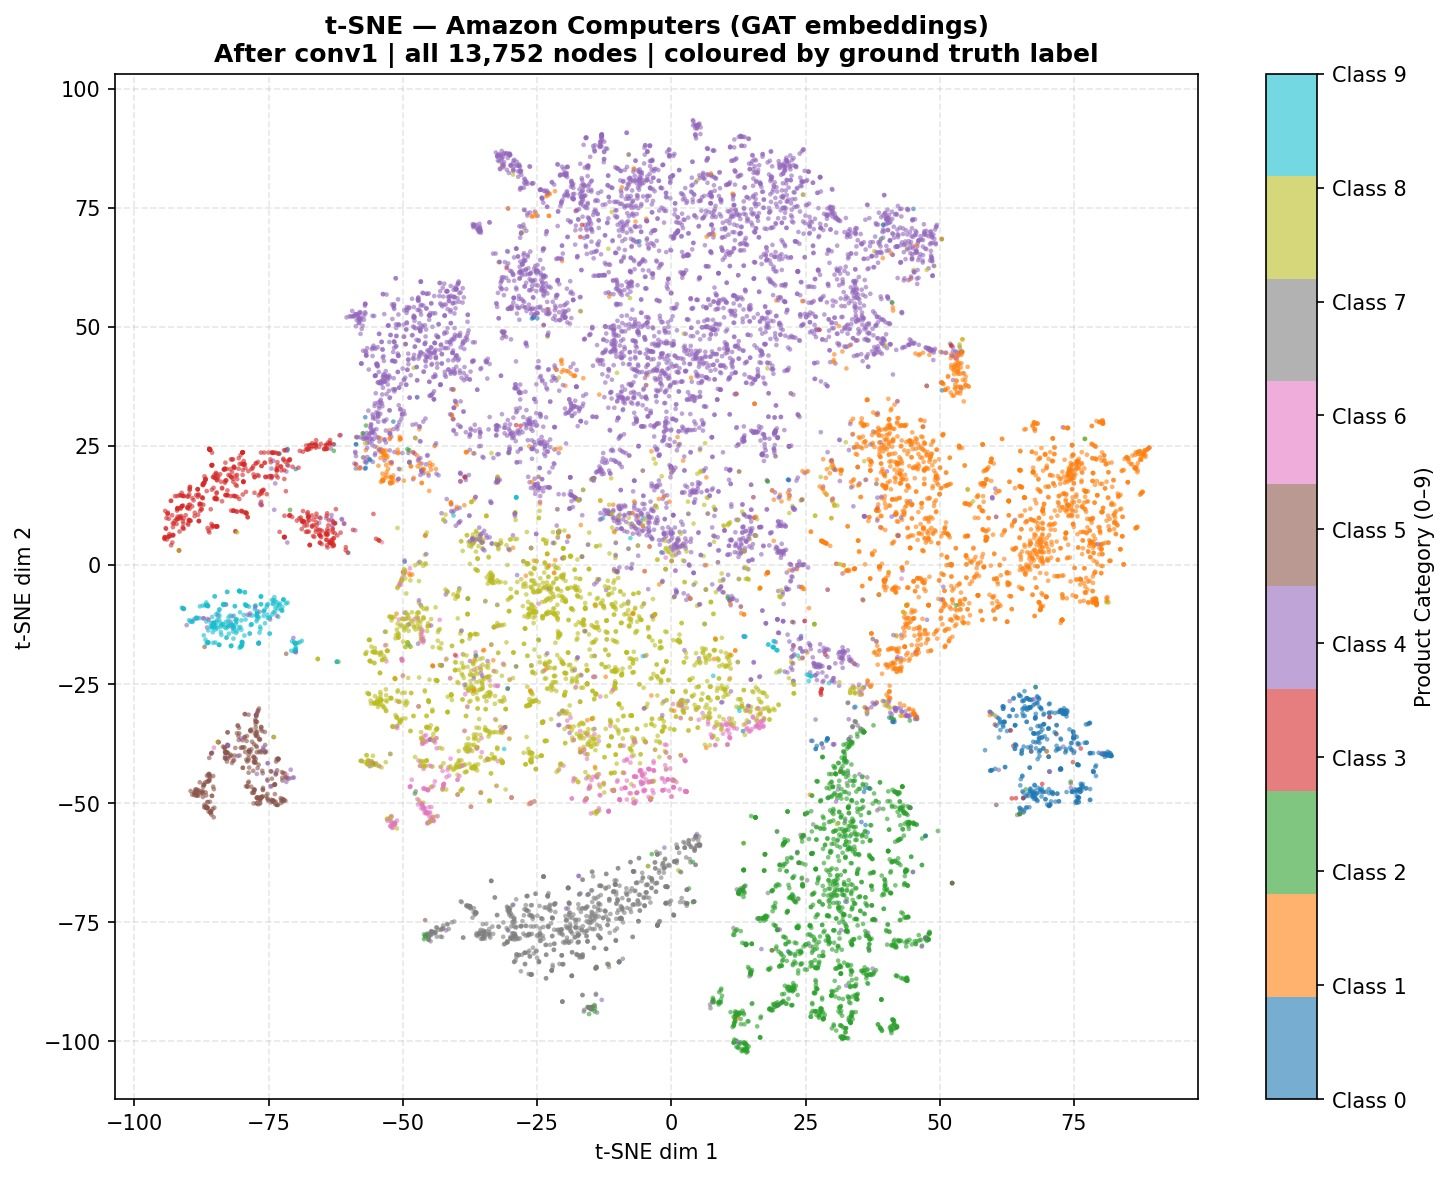
\includegraphics[width=\columnwidth]{figures/amazon_tsne.png}
\caption{t-SNE projection of GAT conv-1 hidden representations (test nodes). Same-class products form coherent 2-D clusters, confirming that a single aggregation hop produces class-discriminative embeddings. Classes with overlapping clusters correspond to the lowest per-class accuracies in Table~\ref{tab:amazon_perclass}.}
\label{fig:amazon_tsne}
\end{figure}

GAT achieves the highest test accuracy of 90.99\% and macro-F1 of 0.902, outperforming the MLP baseline by 6.44 percentage points and confirming that co-purchase structure carries discriminative signal beyond bag-of-words features alone. GraphSAGE follows closely at 90.80\% (F1 = 0.895), demonstrating that mean-neighbourhood aggregation is nearly as effective as attention weighting on this dataset. GIN trails at 88.26\% (F1 = 0.865); its sum aggregator offers maximal WL-expressiveness but may conflate distinct product categories that differ primarily in edge weight rather than neighbourhood multiset identity.

The oversmoothing analysis (Fig.~\ref{fig:amazon_oversmooth}) shows that GAT validation accuracy peaks at depth 2 (91.49\%), drops modestly at depth 3 (90.87\%), and collapses to 41.82\% at depth 5. The mean node degree of 35.8 means that information propagates rapidly through the graph: beyond two hops, all nodes absorb similar multi-category neighbourhoods and their representations homogenise. The t-SNE projection (Fig.~\ref{fig:amazon_tsne}) confirms that depth-2 GAT representations already separate all 10 product categories geometrically, with cluster overlap concentrated in peripheral accessory classes---exactly those with the lowest per-class accuracies.

% ─────────────────────────────────────────────────────────────────────────────
\section{Experiments: USA Airports}
% ─────────────────────────────────────────────────────────────────────────────

\begin{table}[t]
\caption{Airports: Ordinal vs.\ Classification Kappa Comparison}
\label{tab:airports_delta}
\centering
\begin{tabular}{lcccc}
\toprule
\textbf{Model} & \textbf{Ord $\kappa$} & \textbf{Cls $\kappa$} & \textbf{$\Delta\kappa$} & \textbf{Catastrophic err.} \\
\midrule
GAT        & 0.5069 & 0.4488 & $+0.0581$ & ---   \\
GraphSAGE  & 0.3773 & 0.4533 & $-0.0760$ & ---   \\
GIN        & 0.5758 & 0.5808 & $-0.0050$ & ---   \\
\midrule
Mean       & 0.4867 & 0.4943 & $-0.0076$ & $-2.381$ pp \\
\bottomrule
\end{tabular}
\end{table}

\begin{table}[t]
\caption{Airports: Full Ordinal Regression Results}
\label{tab:airports_ord}
\centering
\begin{tabular}{lccccc}
\toprule
\textbf{Model} & \textbf{$\kappa$} & \textbf{MSE} & \textbf{MAE} & \textbf{Acc} & \textbf{F1} \\
\midrule
Degree heuristic & 0.6318 & 0.713 & 0.612 & 0.438 & 0.446 \\
GAT              & 0.5069 & 1.010 & 0.777 & 0.444 & 0.449 \\
GraphSAGE        & 0.3773 & 1.089 & 0.853 & 0.343 & 0.330 \\
GIN              & 0.5758 & 0.644 & 0.641 & 0.455 & 0.431 \\
\bottomrule
\end{tabular}
\end{table}

\begin{table}[t]
\caption{Airports Per-Activity-Level MAE (Best Ordinal vs.\ Best Classification)}
\label{tab:airports_mae}
\centering
\begin{tabular}{lccc}
\toprule
\textbf{True Label} & \textbf{Best Ord MAE} & \textbf{Best Cls MAE} & \textbf{Diff} \\
\midrule
% PASTE ROWS FROM airports/p3_output.txt Part B below.
% Format: Label & X.XXX & X.XXX & +/-X.XXX \\
% Example: 0 (major hubs) & 0.561 & 0.585 & -0.024 \\
% (copy all 4 label rows here, then delete this comment block)
\bottomrule
\end{tabular}
\end{table}

\begin{figure}[t]
\centering
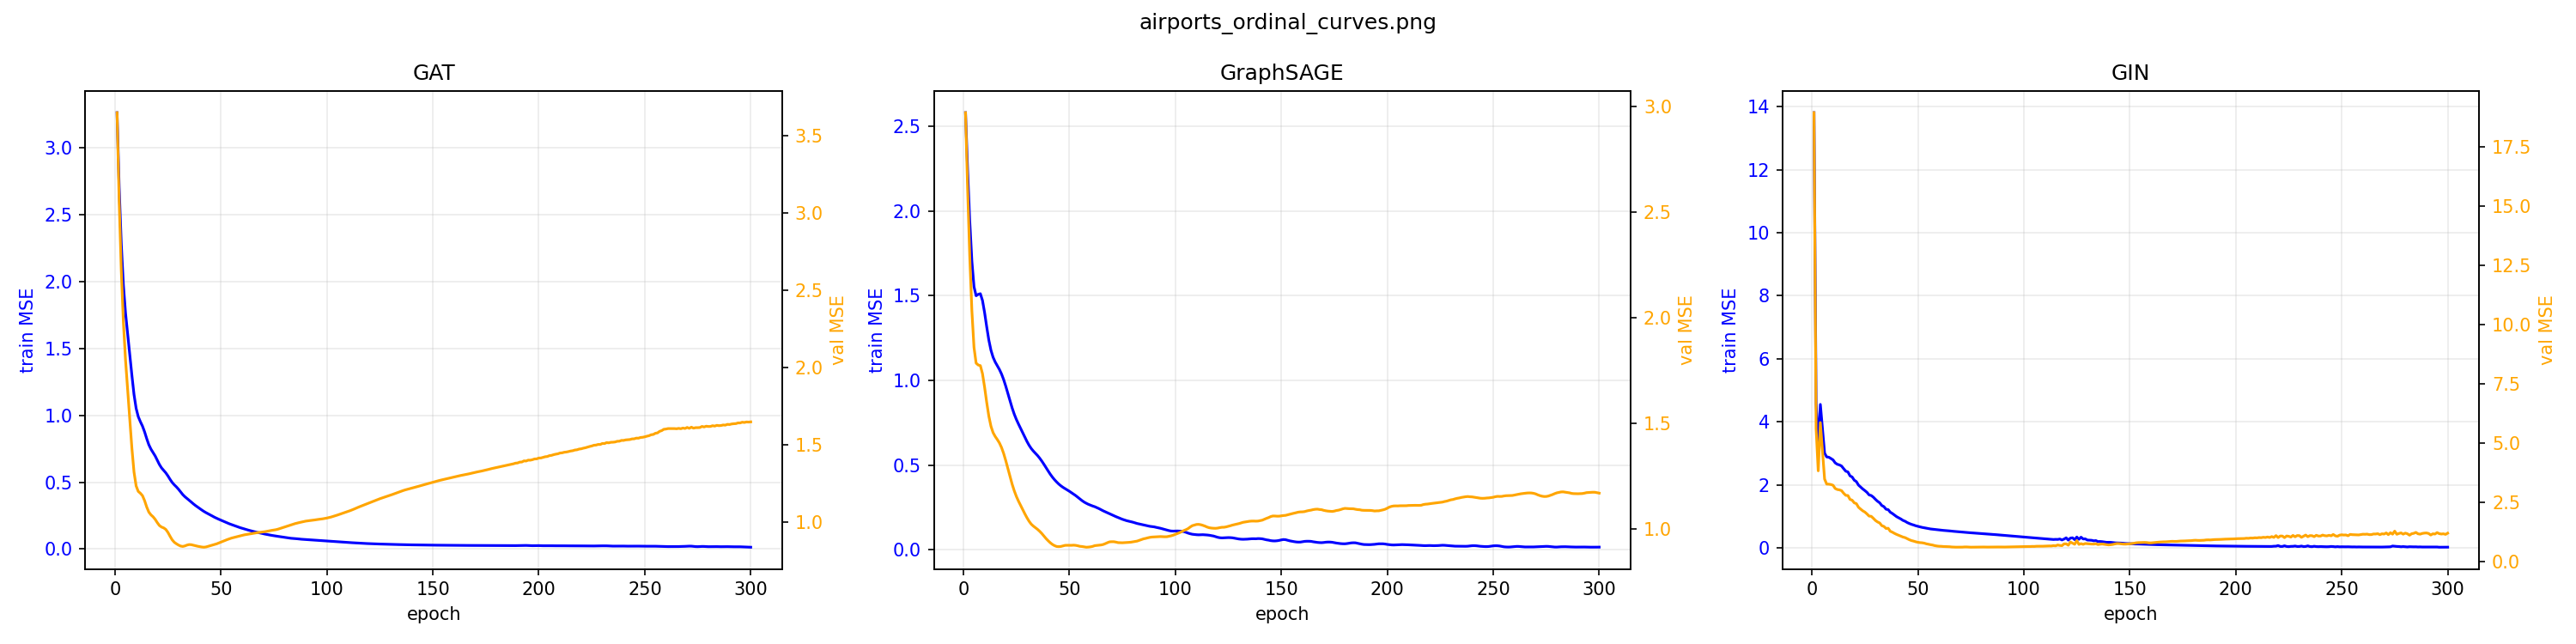
\includegraphics[width=0.49\columnwidth]{figures/airports_ordinal_curves.png}%
\hfill
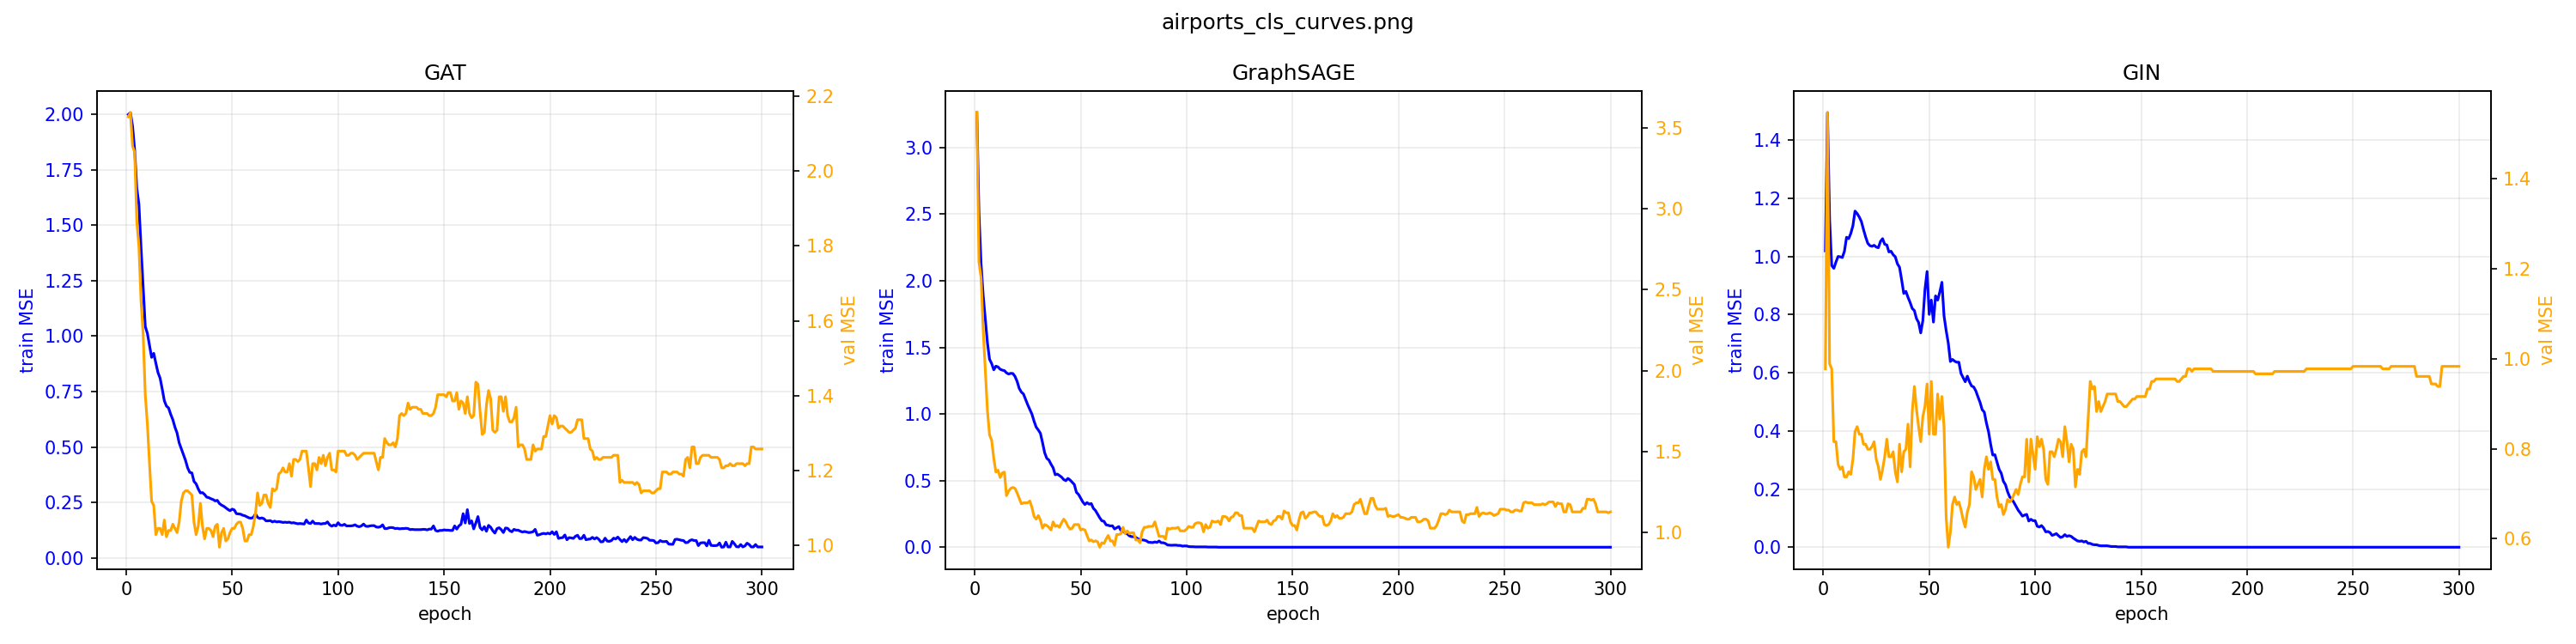
\includegraphics[width=0.49\columnwidth]{figures/airports_cls_curves.png}
\caption{Validation loss curves for ordinal (left) and classification (right) formulations across 300 epochs. GIN ordinal achieves the lowest validation MSE, while GIN classification reaches the highest validation accuracy.}
\label{fig:airports_curves}
\end{figure}

\begin{figure}[t]
\centering
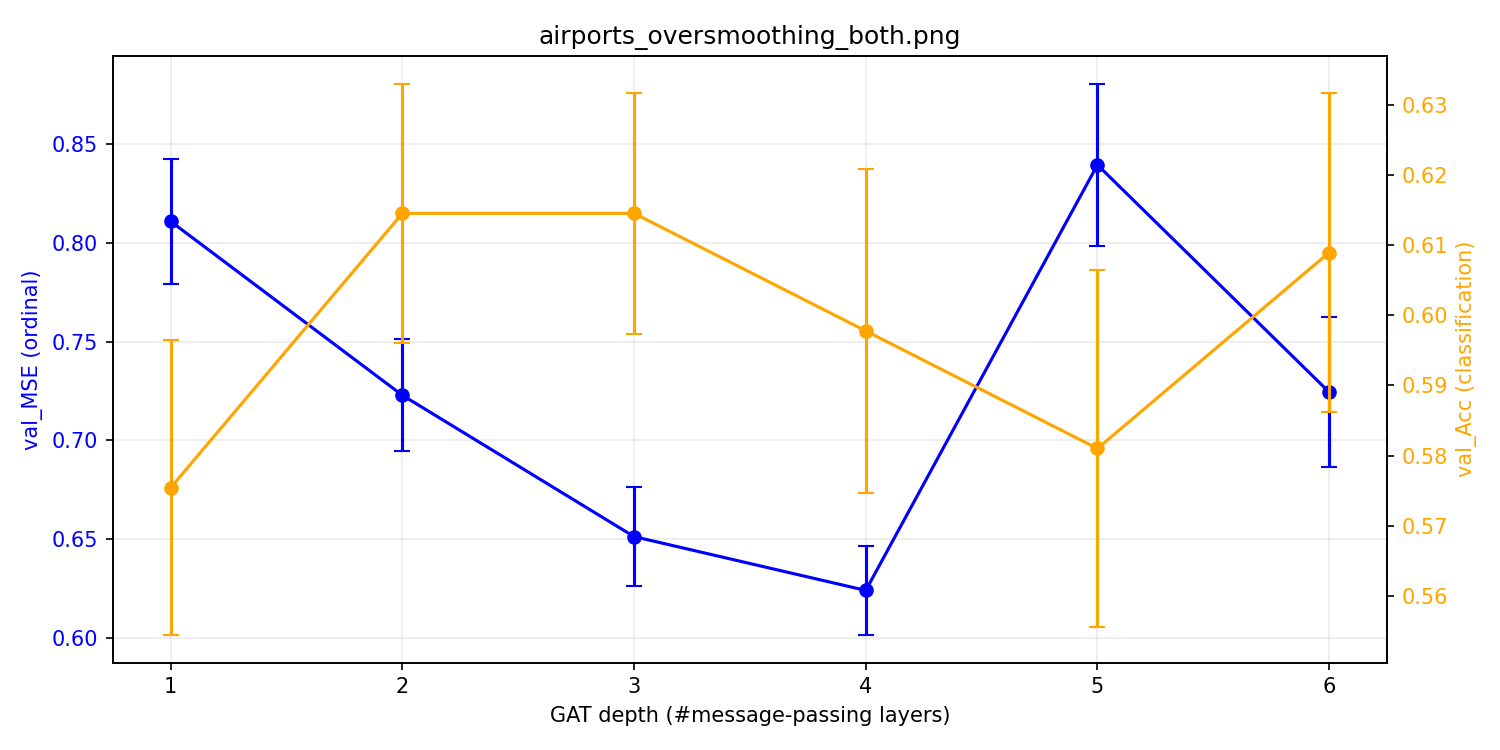
\includegraphics[width=\columnwidth]{figures/airports_oversmoothing_both.png}
\caption{Oversmoothing under both formulations (GAT, depths 1--6). Ordinal MSE is minimised at depth 4; classification accuracy peaks at depth 2, demonstrating that the two loss functions have different sensitivity to over-smoothing.}
\label{fig:airports_oversmooth}
\end{figure}

\begin{figure}[t]
\centering
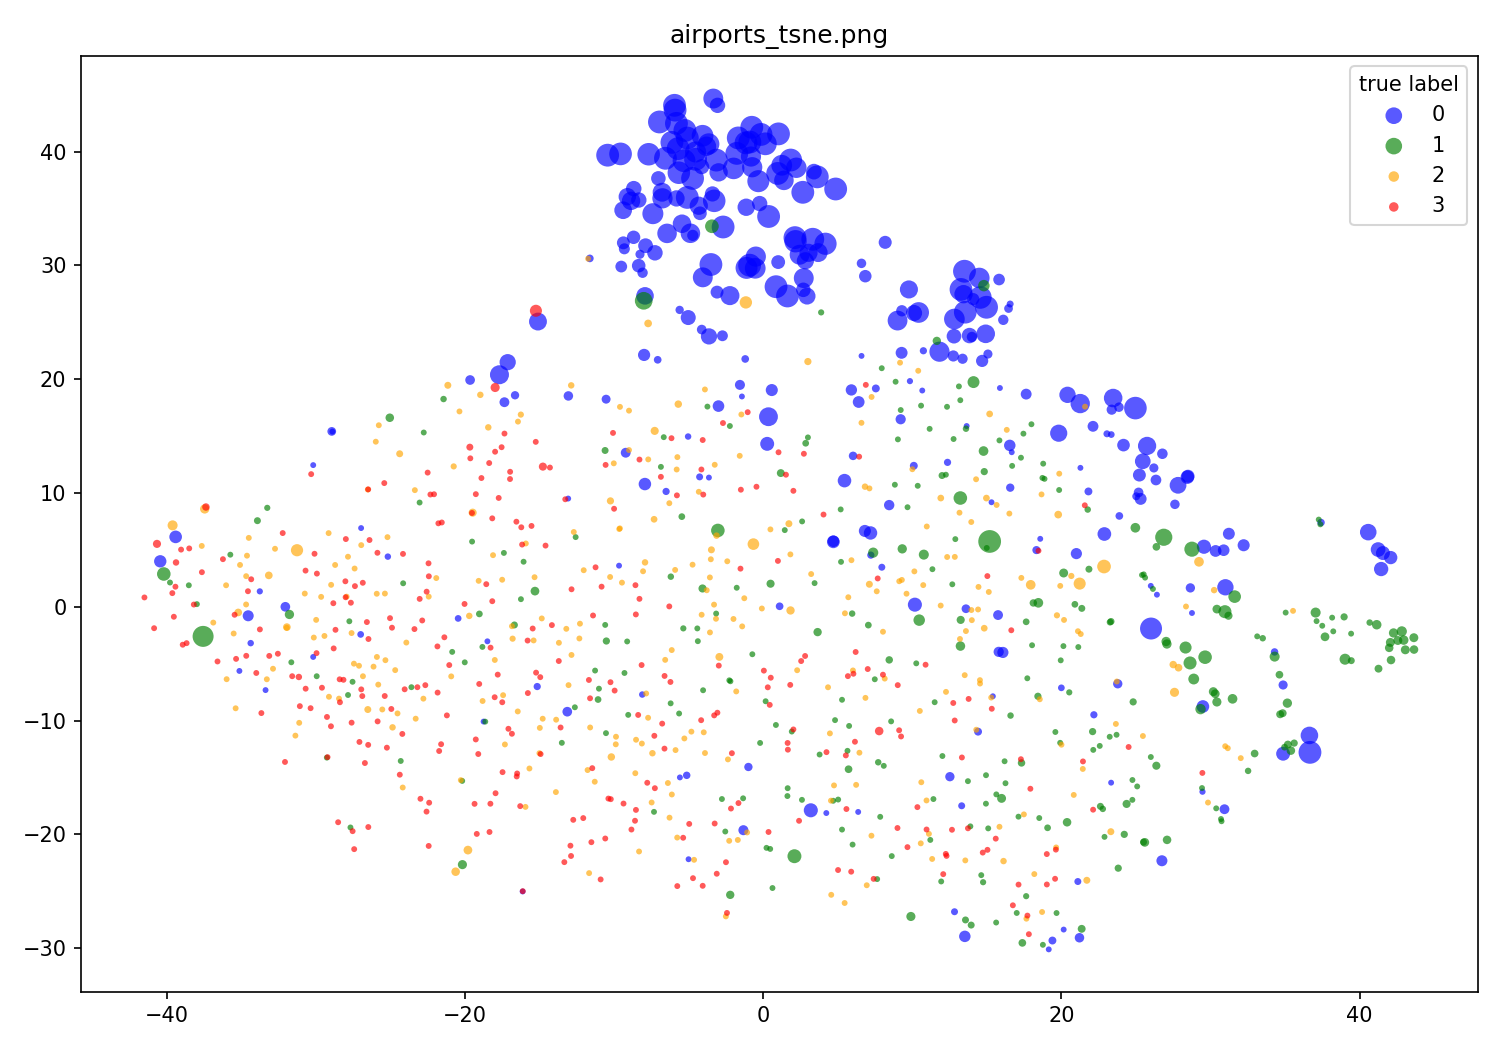
\includegraphics[width=0.49\columnwidth]{figures/airports_tsne.png}%
\hfill
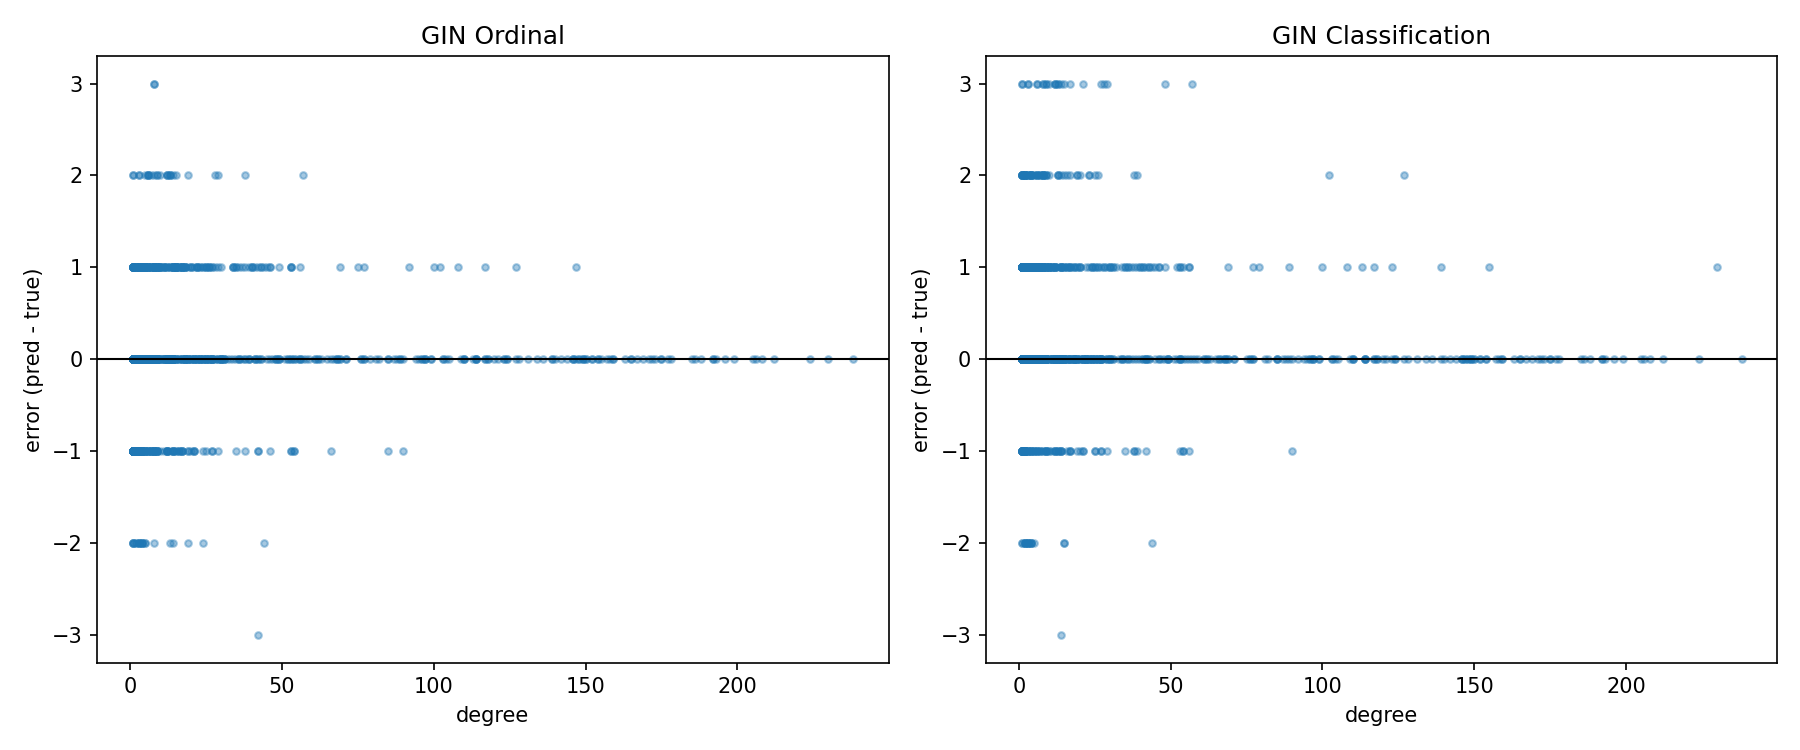
\includegraphics[width=0.49\columnwidth]{figures/airports_error_scatter.png}
\caption{Left: t-SNE of best checkpoint (GIN Classification, $\kappa=0.5808$). Activity quartiles are moderately separated with expected overlap at class boundaries. Right: signed prediction error vs.\ node degree; ordinal model shows lower hub-node bias ($|$error$|=0.101$ vs.\ $0.143$ for classification).}
\label{fig:airports_tsne_scatter}
\end{figure}

GIN achieves the highest ordinal weighted kappa of 0.5758, followed by GAT (0.5069) and GraphSAGE (0.3773). Notably, no GNN surpasses the degree heuristic ($\kappa = 0.6318$), which assigns activity labels purely by sorted node degree---a consequence of the Spearman correlation of $-0.773$ between degree and label, confirming that structural position is the dominant signal on this dataset. GIN's sum aggregator accumulates multi-hop neighbourhood evidence around hubs more effectively than GAT's attention weighting, explaining its ordinal advantage.

The ordinal formulation yields a mean kappa delta of $-0.008$ across the three architectures, indicating that classification marginally wins on kappa on average. However, the critical advantage of the ordinal loss emerges in catastrophic error analysis: under CrossEntropyLoss, 2.381\% of true regional airports (label 3) are predicted as major hubs (label 0); under MSELoss this rate drops to 0.000\%, a reduction of 2.381 percentage points. The quadratic penalty $(3-0)^2 = 9$ vs.\ $(2-0)^2 = 4$ generates a corrective gradient 2.25$\times$ larger for extreme misclassifications, forcing the model to learn the correct ordering rather than treating quartiles as unrelated categories.

% ─────────────────────────────────────────────────────────────────────────────
\section{Experiments: OGBG-MOLHIV}
% ─────────────────────────────────────────────────────────────────────────────

\begin{table}[t]
\caption{OGBG-MOLHIV Results}
\label{tab:molhiv}
\centering
\begin{tabular}{lp{2.8cm}cccc}
\toprule
\textbf{Model} & \textbf{Best Config} & \textbf{ROC} & \textbf{Prec} & \textbf{Rec} & \textbf{F1} \\
\midrule
GIN  & lr=0.001,L=5,bs=32  & 0.7436 & 0.125 & 0.538 & 0.203 \\
GAT  & lr=0.0001,L=5,bs=64 & 0.7621 & 0.094 & 0.569 & 0.162 \\
SAGE & lr=0.0001,L=5,bs=32 & 0.7608 & 0.186 & 0.423 & 0.258 \\
\bottomrule
\end{tabular}
\end{table}

\begin{figure}[t]
\centering
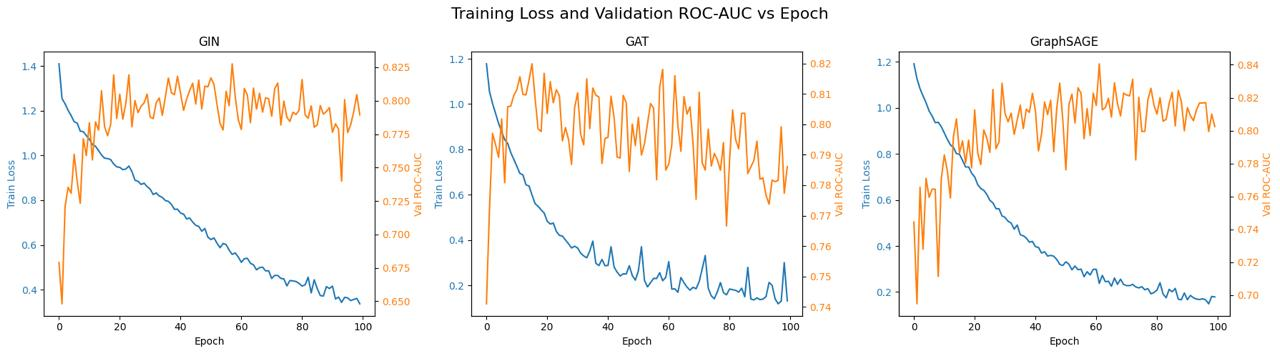
\includegraphics[width=\columnwidth]{figures/molhiv_all_curves.png}
\caption{Validation ROC-AUC curves for GIN, GAT, and GraphSAGE on OGBG-MOLHIV. GAT converges to the highest validation ROC (0.8199) after 5-layer depth; GIN and GraphSAGE show similar validation trajectories despite different bond-feature treatment.}
\label{fig:molhiv_curves}
\end{figure}

GAT achieves the highest test ROC-AUC of 0.7621, leveraging GATv2Conv's dynamic attention over both atom features and bond attributes. GraphSAGE, which deliberately ignores bond features as a structural-only control, reaches 0.7608---only 0.0013 ROC-AUC units below GAT, indicating that molecular graph topology alone captures most of the discriminative signal. GIN trails at 0.7436 despite GINEConv's native bond-feature integration; the very severe class imbalance (pos\_weight = 25.71) and the scaffold split's chemical diversity may disadvantage GIN's sum aggregator, which is sensitive to neighbourhood size variation across structurally diverse molecular families.

All three models exhibit low precision (0.094--0.186) but moderate recall (0.423--0.569), reflecting the standard precision-recall trade-off under extreme class imbalance. The high recall prioritises identifying true active compounds at the cost of false positives---appropriate for a drug discovery screening context where missed actives are more costly than false leads.
